\documentclass[12pt]{article}

\usepackage{amsmath}
\usepackage{amssymb}
\usepackage{bm}
\usepackage{enumerate}
\usepackage{fancyvrb}
\usepackage[top=1in, bottom=1in, left=1in, right=1in]{geometry}
\usepackage{hyperref}
\usepackage{placeins}
\usepackage{tikz}
\usepackage{tikzsymbols}
\usepackage{todonotes}
\usepackage[most]{tcolorbox}
\usepackage{bbm}
\usepackage[thinlines]{easytable}
\usepackage{float}
\usepackage{blindtext,pgffor}

\usetikzlibrary{positioning,calc}

\title{10-703 Deep RL and Controls\\
  Homework 3\\
}


\begin{document}

\maketitle



% \section*{Problem 1}

% \todo[inline]{Show that Bellman backup converges to a fixed point with
% max version of equation.}

\section*{Problem 1}
LQR
\begin{tcolorbox}[breakable, enhanced]	
	Answer: \\
	In this problem, the infinite discrete LQR is implemented. 
	\begin{enumerate}
	\item
	LQR on TWoLinkArm-v0 has the total reward -417.57, steps to reach the goal 411. The $q$, $\dot{q}$ and $u$ plots are in the Figure \ref{fig:lqr_states_1} and \ref{fig:lqr_actions_1}
	
	\begin{figure}[H]
	\caption{LQR on TwoLinkArm-v0: state trajectory}	
	\centering
	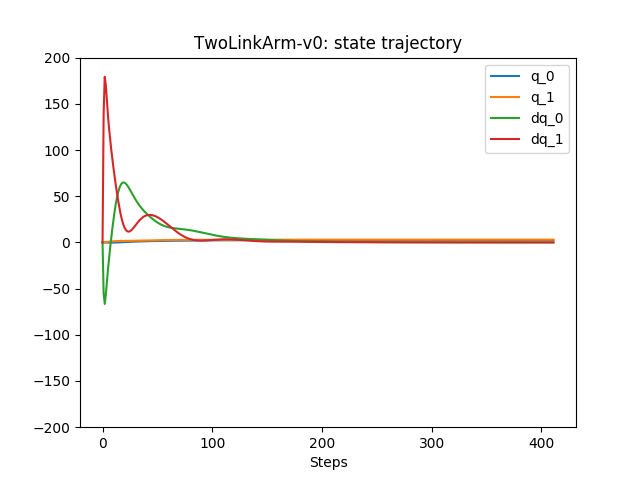
\includegraphics[width=0.8\textwidth]{lqr_1_states.png}
	\label{fig:lqr_states_1}
	\end{figure}
	
	\begin{figure}[H]
	\caption{LQR on TwoLinkArm-v0: raw action trajectory}
	\centering
	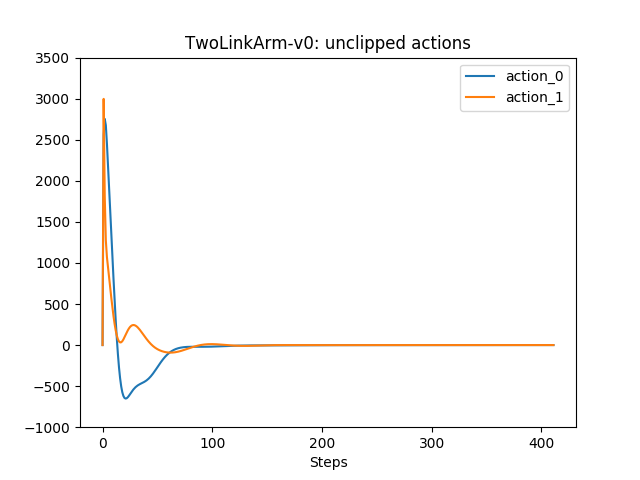
\includegraphics[width=0.8\textwidth]{lqr_1_raw_acts.png}
	\label{fig:lqr_actions_1}	
	\end{figure}
	
	\item
	LQR on TWoLinkArm-limited-torque-v0 has the total reward -4288.58, steps to reach the goal 1836. The $q$, $\dot{q}$, $u$ and the clipped $u$ plots are in the Figure \ref{fig:lqr_states_2}, \ref{fig:lqr_actions_2}, \ref{fig:lqr_actions_clipped_2}. 
	
	\begin{figure}[H]
	\caption{LQR on TwoLinkArm-limited-torque-v0: state trajectory}	
	\centering
	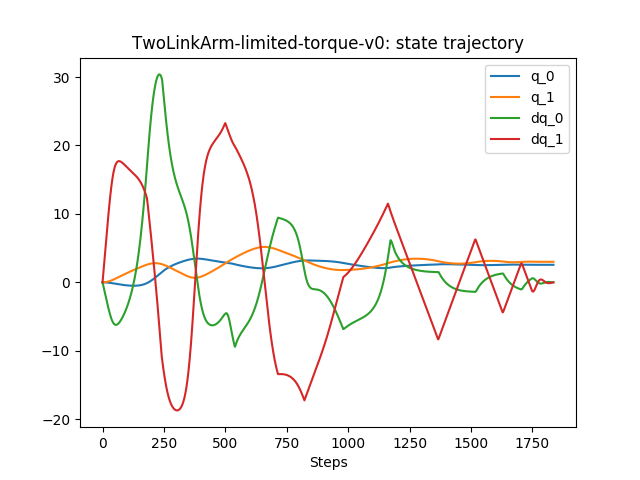
\includegraphics[width=0.8\textwidth]{lqr_2_states.png}
	\label{fig:lqr_states_2}
	\end{figure}
	
	\begin{figure}[H]
	\caption{LQR on TwoLinkArm-limited-torque-v0: raw action trajectory}
	\centering
	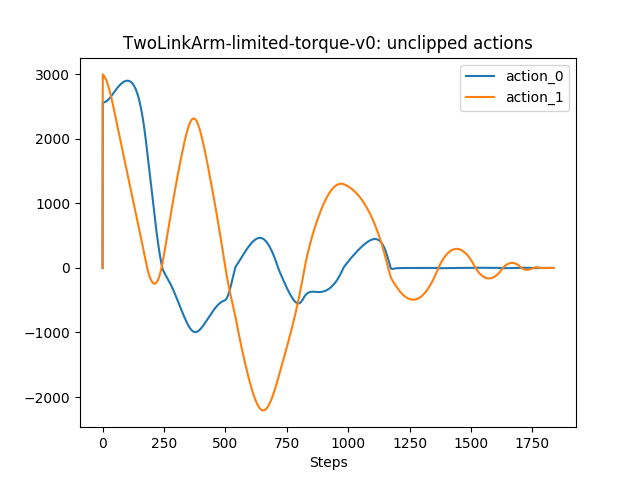
\includegraphics[width=0.8\textwidth]{lqr_2_raw_acts.png}
	\label{fig:lqr_actions_2}	
	\end{figure}
	
	\begin{figure}[H]
	\caption{LQR on TwoLinkArm-limited-torque-v0: clipped action trajectory}
	\centering
	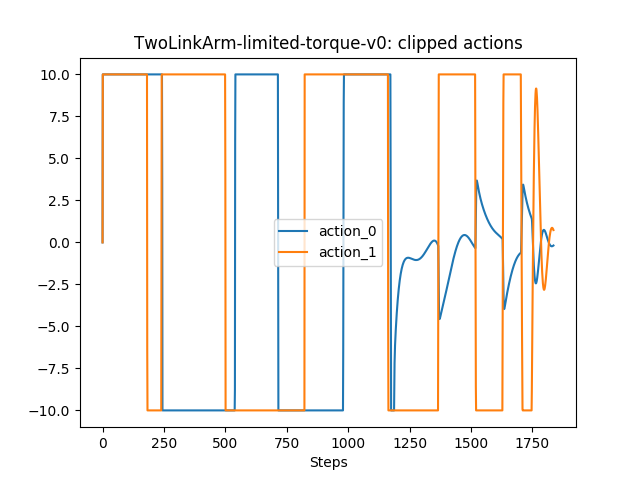
\includegraphics[width=0.8\textwidth]{lqr_2_clipped_acts.png}
	\label{fig:lqr_actions_clipped_2}	
	\end{figure}
	
	\item
	Under the TwoLinkArm-v0 environment where the torque is unlimited, the lqr controller can soon make the arm reach the goal state because unlimited torque can be forced to the arm. As shown in the Figure \ref{fig:lqr_actions_1}, the torque can reach to 3000 for the TwoLinkArm-v0 environment. As the results, the $\dot{q}$ can be more than 150, as shown in the Figure \ref{fig:lqr_states_1}. It may be hard to see in the Figure \ref{fig:lqr_states_1}, the $q$ reaches the goal smoothly with little oscillations. 
	
	Under the TwoLinkArm-limited-torque-v0 environment where the torque is limited to 10 and -10, the LQR controller needs much longer time to make the arms reach the goal state. However, because the torque is limited, the $\dot{q}$ is always small, as shown in Figure \ref{fig:lqr_states_2}. Compared to the TwoLineArm-v0, there are obvious oscillations for the $q$ before it converges to the goal, as shown in the Figure \ref{fig:lqr_states_2}. 
	
	\item
	LQR on TWoLinkArm-v1 has the total reward -2405.65, steps to reach the goal 1844. The $q$, $\dot{q}$ and $u$ plots are in the Figure \ref{fig:lqr_states_4} and \ref{fig:lqr_actions_4}
	
	\begin{figure}[H]
	\caption{LQR on TwoLinkArm-v1: state trajectory}	
	\centering
	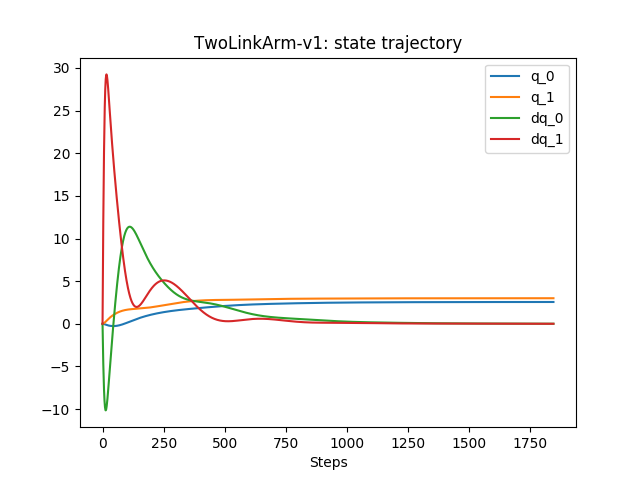
\includegraphics[width=0.8\textwidth]{lqr_4_states.png}
	\label{fig:lqr_states_4}
	\end{figure}
	
	\begin{figure}[H]
	\caption{LQR on TwoLinkArm-v1: raw action trajectory}
	\centering
	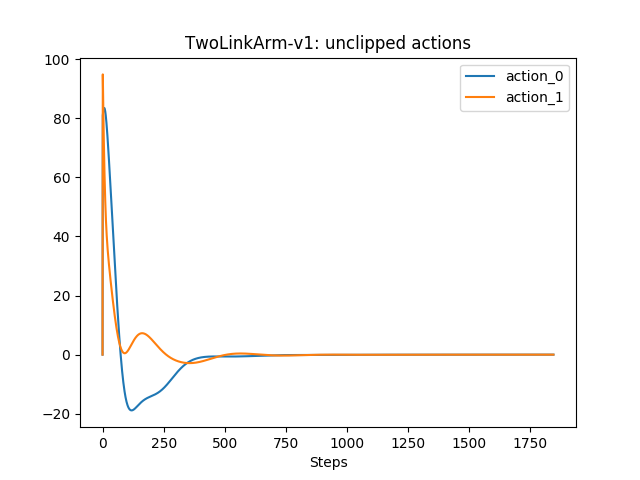
\includegraphics[width=0.8\textwidth]{lqr_4_raw_acts.png}
	\label{fig:lqr_actions_4}	
	\end{figure}
	
	\item
	LQR on TWoLinkArm-limited-torque-v1 has the total reward -3249.94, steps to reach the goal 1950. The $q$, $\dot{q}$, $u$ and the clipped $u$ plots are in the Figure \ref{fig:lqr_states_5}, \ref{fig:lqr_actions_5}, \ref{fig:lqr_actions_clipped_5}. 
	
	\begin{figure}[H]
	\caption{LQR on TwoLinkArm-limited-torque-v1: state trajectory}	
	\centering
	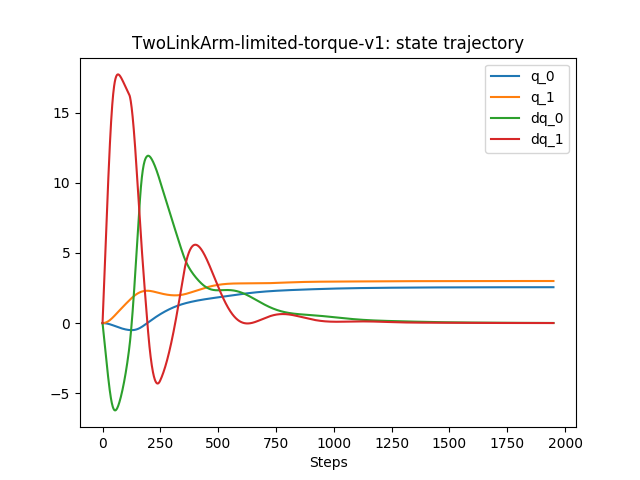
\includegraphics[width=0.8\textwidth]{lqr_5_states.png}
	\label{fig:lqr_states_5}
	\end{figure}
	
	\begin{figure}[H]
	\caption{LQR on TwoLinkArm-limited-torque-v1: raw action trajectory}
	\centering
	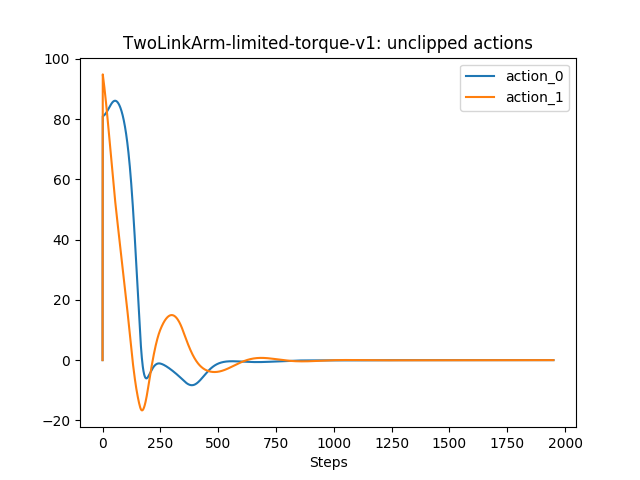
\includegraphics[width=0.8\textwidth]{lqr_5_raw_acts.png}
	\label{fig:lqr_actions_5}	
	\end{figure}
	
	\begin{figure}[H]
	\caption{LQR on TwoLinkArm-limited-torque-v1: clipped action trajectory}
	\centering
	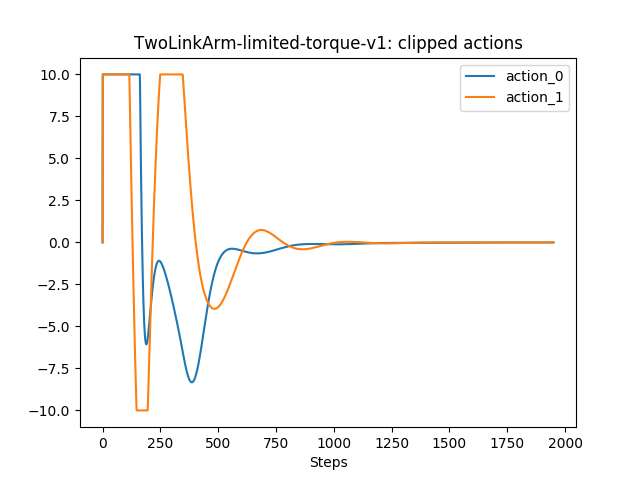
\includegraphics[width=0.8\textwidth]{lqr_5_clipped_acts.png}
	\label{fig:lqr_actions_clipped_5}	
	\end{figure}
	
	\item
	For TwoLinkArm-v1, the action trajectory has the similar shape as its v0 version, but the magnitude is much less than the v0 version because $u$ has larger penalty in v1. Basically, the action plot of the v1 (Figure \ref{fig:lqr_actions_4}) is like a horizontally streched and vertically compressed version of Figure \ref{fig:lqr_actions_1}. As the results, the state trajectory of the v1 version is also like a horizontally streched and vertically compressed version of Figure \ref{fig:lqr_states_1}. Therefore, the total reward of v1 is much smaller and the total step is much larger than the v0 version. 
	
	For TwoLinkArm-limite-torque-v1, its state action trajectory looks very different from its v0 version, probably because the raw action from LQR is much smaller than v0 and there are less actions to be clipped. Therefore, the state trajectory of the v1 version reaches the goal with much less oscillations than the v0 version. Also, the actions of the v1 version are generally smaller than the v0 version. As the results, the total reward of the v1 version is much higher than the v0 version, even though the number of steps to reach the goal is similar. 
	\end{enumerate}
\end{tcolorbox}

\section*{Problem 2}
Linear Q-network (no experience replay or target fixing)
\begin{tcolorbox}[breakable, enhanced]	
	Answer:	
	\begin{center}
	\begin{enumerate}

\item
	{\bf Experiement setup:} 
	
\begin{table}[H]
\centering
\caption{LQN Experiement setup}
\label{dqn:hyperpara}
\begin{tabular}{|l|l|l|}
\hline
\textbf{Hyperparameter} & \textbf{Value} & \textbf{Note} \\ \hline
environment & Enduro-v0 &  \\ \hline
minibatch size & 32 & Follow {[}2{]} \\ \hline
has replay memory? & False &  \\ \hline
agent history length & 4 & Follow {[}2{]} \\ \hline
discount factor & 0.99 & Follow {[}2{]} \\ \hline
action repeat & \begin{tabular}[c]{@{}l@{}}Uniform random \\ 2, 3 or 4\end{tabular} & \begin{tabular}[c]{@{}l@{}}Default by the Openai \\ Gym Enduro-v0 \\ environment\end{tabular} \\ \hline
update frequency & Every 4 steps & Follow {[}2{]} \\ \hline
learning rate & 0.0001 &  \\ \hline
optimizer & Adam &  \\ \hline
adam-beta1 & 0.9 & Tensorflow default \\ \hline
adam-beta2 & 0.999 & Tensorflow default \\ \hline
adam-epsilon & 1e-08 & Tensorflow default \\ \hline
initial exploration & 1.0 & Follow [2] \\ \hline
final exploration & 0.05 & Follow [2] \\ \hline
\begin{tabular}[c]{@{}l@{}}exploration linear\\ decay steps\end{tabular} & 1M & Follow [2] \\ \hline
game frame dim & 110*84 & \begin{tabular}[c]{@{}l@{}}\end{tabular} \\ \hline
\end{tabular}
\end{table}
 
\item {\bf Learning curve}


The evalution reward of the LQN is zero for the first 1.50M steps, and then fluctuates above zero. The evaluation reward near the end of learning is still close to zero. This may indicate that the simple LQN cannot learn the game well. 

\item {\bf Final evaluation reward:}

100-episode greedy policy: $19.69 \pm 1.05$

	
	\end{enumerate}
	\end{center}	
\end{tcolorbox}

\section*{Problem 3}
Linear Q-network with experience replay and target fixing
\begin{tcolorbox}	
	Answer:	
	\begin{center}

	\end{center}	
\end{tcolorbox}

\section*{Problem 4}
Linear double Q-network 
\begin{tcolorbox}	
	Answer:	
	\begin{center}
	
	\end{center}	
\end{tcolorbox}
\section*{Problem 5}
Deep Q-network
\begin{tcolorbox}[breakable, enhanced]
	
	Answer:	
	\begin{center}
	\begin{enumerate}
	\item
	{\bf Experiement setup:} 
	
\begin{table}[H]
\centering
\caption{DQN Experiement setup}
\label{dqn:hyperpara}
\begin{tabular}{|l|l|l|}
\hline
\textbf{Hyperparameter} & \textbf{Value} & \textbf{Note} \\ \hline
environment & Enduro-v0 &  \\ \hline
minibatch size & 32 & Follow {[}2{]} \\ \hline
has replay memory? & True &  \\ \hline
replay memory size & 500000 & \begin{tabular}[c]{@{}l@{}}For memory consideration, \\ to ensure not reach memory \\ limit of the Bridges cluster.\end{tabular} \\ \hline
agent history length & 4 & Follow {[}2{]} \\ \hline
discount factor & 0.99 & Follow {[}2{]} \\ \hline
action repeat & \begin{tabular}[c]{@{}l@{}}Uniform random \\ 2, 3 or 4\end{tabular} & \begin{tabular}[c]{@{}l@{}}Default by the Openai \\ Gym Enduro-v0 \\ environment\end{tabular} \\ \hline
update frequency & Every 4 steps & Follow {[}2{]} \\ \hline
learning rate & 0.0001 &  \\ \hline
optimizer & Adam &  \\ \hline
adam-beta1 & 0.9 & Tensorflow default \\ \hline
adam-beta2 & 0.999 & Tensorflow default \\ \hline
adam-epsilon & 1e-08 & Tensorflow default \\ \hline
initial exploration & varies & \begin{tabular}[c]{@{}l@{}}See "Non-continuous learn" \\ part for more\end{tabular} \\ \hline
final exploration & varies & \begin{tabular}[c]{@{}l@{}}See "Non-continuous learn"\\ part for more\end{tabular} \\ \hline
\begin{tabular}[c]{@{}l@{}}exploration linear\\ decay steps\end{tabular} & varies & \begin{tabular}[c]{@{}l@{}}See "Non-continuous learn" \\ part for more\end{tabular} \\ \hline
replay start size & varies & \begin{tabular}[c]{@{}l@{}}See "Non-continuous learn" \\ part for more
\end{tabular} \\ \hline
game frame dim & 110*84 & \begin{tabular}[c]{@{}l@{}}\end{tabular} \\ \hline
\end{tabular}
\end{table}

The convoluted neural network has the same architecture as the [1], in which the first hidden layer has 16 8*8 filters with stride 4 and rectifier activation, the second hidden layer has 32 4*4 filters with stride 2 and rectifier activation, the final hidden layer is a fully connected layer with 256 rectifier activation units, the ouput layer is a fully connected linear layer with the output dimension the same as the environment action number. 
\item 
{\bf Non-continuous learn:}

Because of the limited computing resources on the Bridges clusters, the complete learning process (interact with the environment for 5M steps) may take tens of hours. To speed up the queuing on the Bridges clusters, the learning is segmented into 5 parts. The learned model parameter values of each parts are written into file and imported into the next part as the model initial values. Because the replay memory of each learning part is not remembered, some hyperparameters listed in the table \ref{dqn:hyperpara} need to be tweaked for each learning part, as show in table \ref{dqn:noncont}. It is awared by the authors that the learning behavior of such non-continuous learning may be different from the continuous learning because at each time a new learning part starts, samples in the replay memory have to be recollected. But learning results are reasonble as will be discussed in the following. To mimic the continuous simulation settings, during the non-continuous learning, the initial exploration probablity and the replay start size are decreasing from the first learning part to the last learning part. 

\begin{table}[H]
\centering
\caption{DQN non-continuous learning setup}
\label{dqn:noncont}
\begin{tabular}{|l|l|l|l|l|l|}
\hline
\textbf{} & \textbf{Part 1} & \textbf{Part 2} & \textbf{Part 3} & \textbf{Part 4} & \textbf{Part 5} \\ \hline
\textbf{initial exploration} & 0.5 & 0.35 & \begin{tabular}[c]{@{}l@{}}0.5 \\ (intend for\\ more\\ exploration\\ since \\ evaluation \\ reward is \\ still not \\ good)\end{tabular} & 0.1 & 0.05 \\ \hline
\textbf{final exploration} & 0.05 & 0.05 & 0.05 & 0.05 & 0.05 \\ \hline
\textbf{\begin{tabular}[c]{@{}l@{}}exploration \\ linear decay steps\end{tabular}} & 1M & 700K & 300K & 10K & N/A \\ \hline
\textbf{replay start size} & 50K & 50K & 50K & 10K & 1000 \\ \hline
\textbf{\begin{tabular}[c]{@{}l@{}}final step reached\\ of this part\end{tabular}} & 480K & 450K & 630K & 1.33M & 1.88M \\ \hline
\textbf{\begin{tabular}[c]{@{}l@{}}total step reached\\ of the learning\end{tabular}} & 480K & 930K & 1.56M & 2.89M & 4.77M \\ \hline
\end{tabular}
\end{table}

\item 
{\bf Learning curve:}


The evalution reward of the DQN is zero for the first 500K steps, and then increases with lots of fluctuations. It is reasonble for the agent the learn something after so many interactions with the environment, since gaining the reward requires the agent to continuously speed up until passing some cars. The evaluation reward near the end of learning is around 200.  

\item {\bf Final evaluation reward:}

100-episode greedy policy: $165.28 \pm 4.40$

	\end{enumerate}
	\end{center}	
\end{tcolorbox}
\section*{Problem 6}
Double deep Q-network 
\begin{tcolorbox}[breakable, enhanced]	
	Answer:	
	\begin{center}
	\begin{enumerate}
	\item
	{\bf Experiement setup:} 
	
\begin{table}[H]
\centering
\caption{DDQN Experiement setup}
\label{ddqn:hyperpara}
\begin{tabular}{|l|l|l|}
\hline
\textbf{Hyperparameter} & \textbf{Value} & \textbf{Note} \\ \hline
environment & Enduro-v0 &  \\ \hline
minibatch size & 32 & Follow {[}2{]} \\ \hline
has replay memory? & True &  \\ \hline
replay memory size & 500000 & \begin{tabular}[c]{@{}l@{}}For memory consideration, \\ to ensure not reach memory \\ limit of the Bridges cluster.\end{tabular} \\ \hline
agent history length & 4 & Follow {[}2{]} \\ \hline
discount factor & 0.99 & Follow {[}2{]} \\ \hline
action repeat & \begin{tabular}[c]{@{}l@{}}Uniform random \\ 2, 3 or 4\end{tabular} & \begin{tabular}[c]{@{}l@{}}Default by the Openai \\ Gym Enduro-v0 \\ environment\end{tabular} \\ \hline
update frequency & Every 4 steps & Follow {[}2{]} \\ \hline
target net update frequency & \begin{tabular}[c]{@{}l@{}}Every 10000 updates \\ (every 40000 steps) \end{tabular} & Follow {[}2{]} \\ \hline
learning rate & 0.0001 &  \\ \hline
optimizer & Adam &  \\ \hline
adam-beta1 & 0.9 & Tensorflow default \\ \hline
adam-beta2 & 0.999 & Tensorflow default \\ \hline
adam-epsilon & 1e-08 & Tensorflow default \\ \hline
initial exploration & varies & \begin{tabular}[c]{@{}l@{}}See "Non-continuous learn" \\ part for more\end{tabular} \\ \hline
final exploration & varies & \begin{tabular}[c]{@{}l@{}}See "Non-continuous learn"\\ part for more\end{tabular} \\ \hline
\begin{tabular}[c]{@{}l@{}}exploration linear\\ decay steps\end{tabular} & varies & \begin{tabular}[c]{@{}l@{}}See "Non-continuous learn" \\ part for more\end{tabular} \\ \hline
replay start size & varies & \begin{tabular}[c]{@{}l@{}}See "Non-continuous learn" \\ part for more
\end{tabular} \\ \hline
game frame dim & 110*84 & \begin{tabular}[c]{@{}l@{}}\end{tabular} \\ \hline
\end{tabular}
\end{table}

The convoluted neural network has the same architecture as the [1], in which the first hidden layer has 16 8*8 filters with stride 4 and rectifier activation, the second hidden layer has 32 4*4 filters with stride 2 and rectifier activation, the final hidden layer is a fully connected layer with 256 rectifier activation units, the ouput layer is a fully connected linear layer with the output dimension the same as the environment action number. 
\item 
{\bf Non-continuous learn:}

Similar to problem 5, the learning is segmented into 6 parts. Some tweaked hyparameters based on the table \ref{ddqn:hyperpara} is shown in the table \ref{ddqn:noncont}. 

\begin{table}[H]
\centering
\caption{DDQN non-continuous learning setup}
\label{ddqn:noncont}
\begin{tabular}{|l|l|l|l|l|l|l|}
\hline
\textbf{} & \textbf{Part 1} & \textbf{Part 2} & \textbf{Part 3} & \textbf{Part 4} & \textbf{Part 5} & \textbf{Part 6} \\ \hline
\textbf{initial exploration} & 0.5 & 0.35 & \begin{tabular}[c]{@{}l@{}}0.5 \\ (intend for\\ more\\ exploration\\ since \\ evaluation \\ reward is \\ still not \\ good)\end{tabular} & 0.1 & 0.05 & 0.05 \\ \hline
\textbf{final exploration} & 0.05 & 0.05 & 0.05 & 0.05 & 0.05 & 0.05\\ \hline
\textbf{\begin{tabular}[c]{@{}l@{}}exploration \\ linear decay steps\end{tabular}} & 1M & 700K & 300K & 10K & N/A & N/A\\ \hline
\textbf{replay start size} & 50K & 50K & 50K & 10K & 1000 & 1000 \\ \hline
\textbf{\begin{tabular}[c]{@{}l@{}}final step reached\\ of this part\end{tabular}} & 300K & 500K & 500K & 370K & 360K & 1.68M \\ \hline
\textbf{\begin{tabular}[c]{@{}l@{}}total step reached\\ of the learning\end{tabular}} & 300K & 800K & 1.30M & 1.67M & 2.03M & 3.71M \\ \hline
\end{tabular}
\end{table}

\item 
{\bf Learning curve:}


The evalution reward of the DDQN is basically zero for the first 1M steps, and then increases faster and with less fluctuations than the DQN case. This may prove that DDQN performs better than DQN in terms of stability and learning speed. The learning does not reach the 5M steps due to the time problem. The evaluation reward near the end of learning is around 400, which is higher than the DQN case even the iteration number is less. There is still an increasing trend in the evaluation rewards when the learning stopped. It can be expected that evluation rewards can increase by more iteractions with the environment.    

\item {\bf Final evaluation reward:}

100-episode greedy policy: $420.17 \pm 8.57$

	\end{enumerate}
	\end{center}	
\end{tcolorbox}
\section*{Problem 7}
Dueling deep Q-network (extended from DDQN in the problem 6)
\begin{tcolorbox}[breakable, enhanced]	
	Answer:	
	\begin{center}
	\begin{enumerate}
	\item
	{\bf Experiement setup:} 
	
	The hyperparameters for the Duel-DDQN are the same as the table \ref{ddqn:hyperpara}.

The convoluted neural network has the same settings as the problem 5 and 6, except there are two seperate fully-connected neural network layers after the second the convoluted neural network. One is for calculating the advantage values, which has 256 rectifier units and action-number of outputs, the other is for calculating the state value, which has 256 recrifier units and 1 output. The state value and advantage values are then combined to give the Q value for each action.  
\item 
{\bf Non-continuous learn:}

Similar to problem 6, the learning is segmented into 6 parts. Some tweaked hyparameters is shown in the table \ref{duel-ddqn:noncont}. 

\begin{table}[H]
\centering
\caption{Duel-DDQN non-continuous learning setup}
\label{duel-ddqn:noncont}
\begin{tabular}{|l|l|l|l|l|l|l|}
\hline
\textbf{} & \textbf{Part 1} & \textbf{Part 2} & \textbf{Part 3} & \textbf{Part 4} & \textbf{Part 5} & \textbf{Part 6} \\ \hline
\textbf{initial exploration} & 0.5 & 0.35 & \begin{tabular}[c]{@{}l@{}}0.5 \\ (intend for\\ more\\ exploration\\ since \\ evaluation \\ reward is \\ still not \\ good)\end{tabular} & 0.1 & 0.05 & 0.05 \\ \hline
\textbf{final exploration} & 0.05 & 0.05 & 0.05 & 0.05 & 0.05 & 0.05\\ \hline
\textbf{\begin{tabular}[c]{@{}l@{}}exploration \\ linear decay steps\end{tabular}} & 1M & 700K & 300K & 10K & N/A & N/A\\ \hline
\textbf{replay start size} & 50K & 50K & 50K & 10K & 1000 & 1000 \\ \hline
\textbf{\begin{tabular}[c]{@{}l@{}}final step reached\\ of this part\end{tabular}} & 390K & 370K & 510K & 330K & 320K & 1.36M \\ \hline
\textbf{\begin{tabular}[c]{@{}l@{}}total step reached\\ of the learning\end{tabular}} & 390K & 760K & 1.25M & 1.58M & 1.90M & 3.26M \\ \hline
\end{tabular}
\end{table}

\item 
{\bf Learning curve:}


The evalution reward of the Duel-DDQN is basically zero for the first 800K steps, and then increases faster with even less fluctuations than the DDQN case. This proves the advantages of the dueling architecture. The learning does not reach the 5M steps due to the time problem. The evaluation reward near the end of learning is around 450, which is higher than the DDQN case even the iteration number is less. At the time the learning stopped, the evaluation rewards have already become steady. It is expected that further learning may not increase the evaluation rewards more. 

\item {\bf Final evaluation reward:}

100-episode greedy policy: $478.81 \pm 7.63$

	\end{enumerate}
	\end{center}	
\end{tcolorbox}

\section*{8. Performance Comparison of the Different Methods}

\begin{tcolorbox}[breakable, enhanced]	
	Answer:	
	\begin{center}
	\begin{table}[H]
\centering
\caption{Performance Comparison of the Different Methods}
\label{cmp}
\begin{tabular}{|l|l|l|l|l|l|}
\hline
\textbf{LQN} & \textbf{LQN-Fixing} & \textbf{DLQN} & \textbf{DQN} & \textbf{DDQN} & \textbf{Duel-DDQN} \\ \hline
$19.69 \pm 1.05$& ?? & ?? & $165.28 \pm 4.40$ & $420 \pm 8.57$ & $478.81 \pm 7.63$  \\ \hline

\end{tabular}
\end{table}

Comments ?????? Basically, for the learning steps, LQN $>$ DQN $>$ DDQN $>$ Duel-DDQN, but the evaluation rewards have the reverse relationship. This shows that Duel-DDQN is more effective than DDQN than DQN and than LQN. 
	\end{center}	
\end{tcolorbox}
% some comments about what is important and is not important. 


\end{document}
